\documentclass[UTF8]{ctexart}
\usepackage{graphicx}
\begin{document}
    \begin{enumerate}
        \item[1]
        针对bilibili网站,我们寻找其中的get请求与post请求\\        
        打开首页时\\
        \includegraphics[scale=0.4]{07-02_1.png}\\
        可以从url看出该get请求返回的数据是搜索框的默认值\\
        而内容包如下\\
        \includegraphics[scale=0.4]{07-02_2.png}\\
        而在登陆时\\
        \includegraphics[scale=0.4]{07-02_3.png}\\
        即服务器在动态的请求验证登录信息\\
        内容包如下\\
        \includegraphics[scale=0.4]{07-02_4.png}\\
        \item[2] 
        我们尝试利用jQuery发送弹幕
        \begin{enumerate}
            \item[2.1]
            在更改前界面如下\\ 
            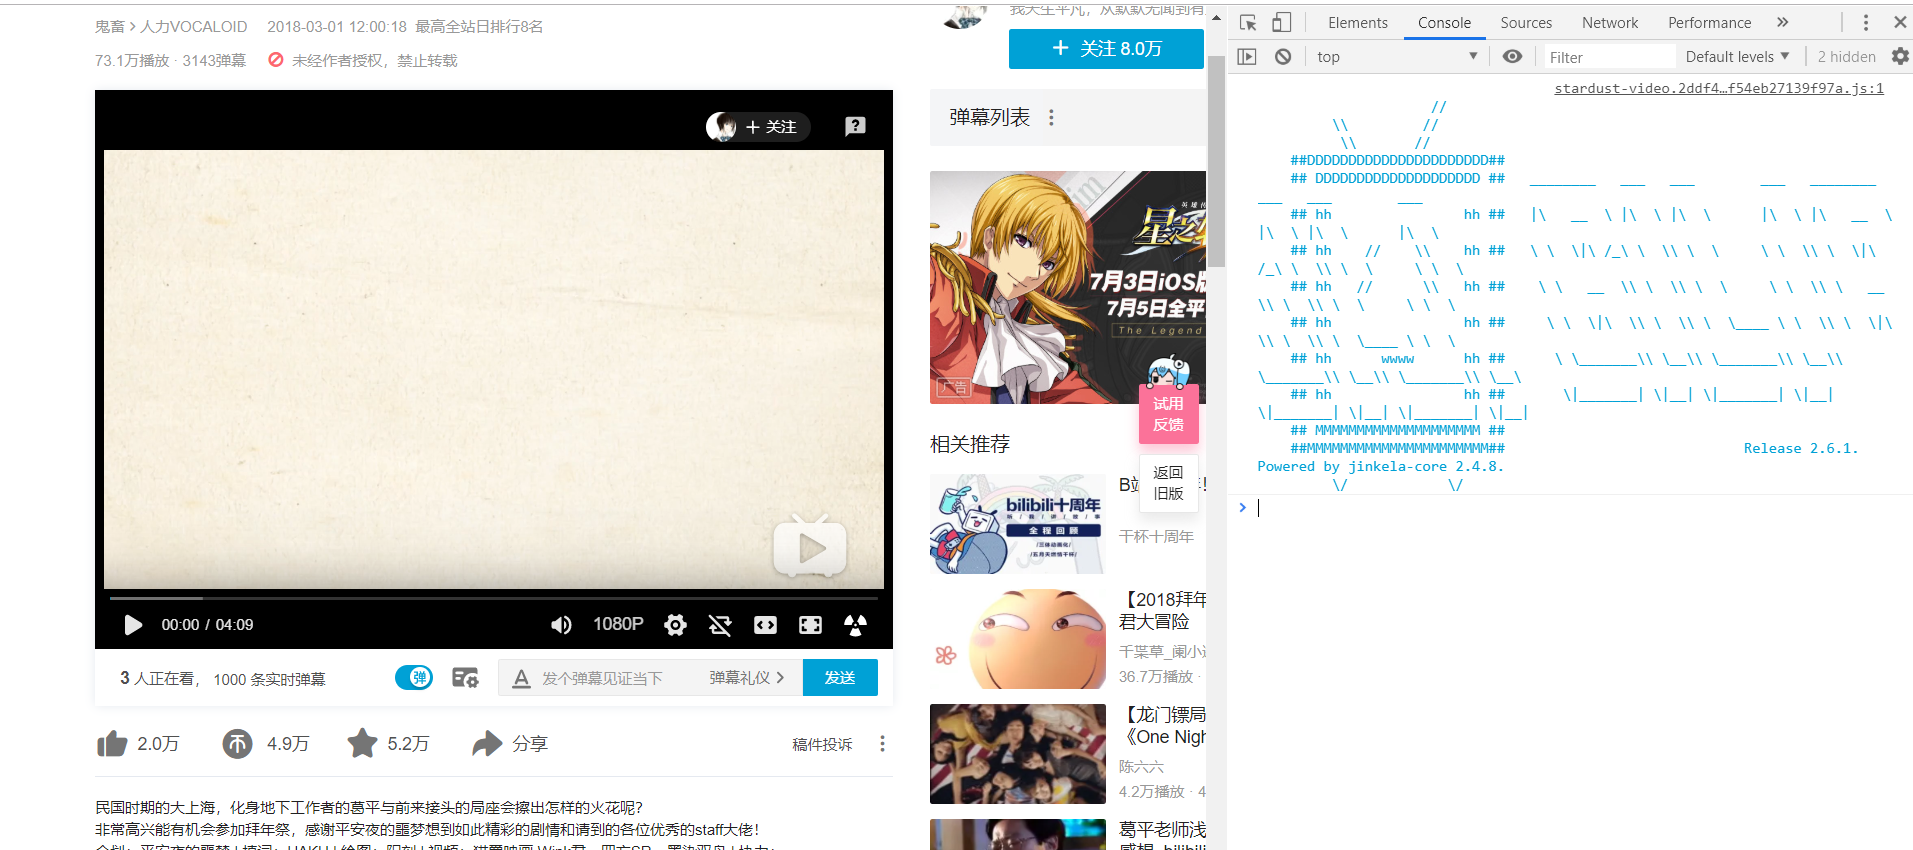
\includegraphics[scale=0.3]{06-27_3.png}
            我们利用类选择器找到想要填充的弹幕内容的input标签,更改它的值\\
            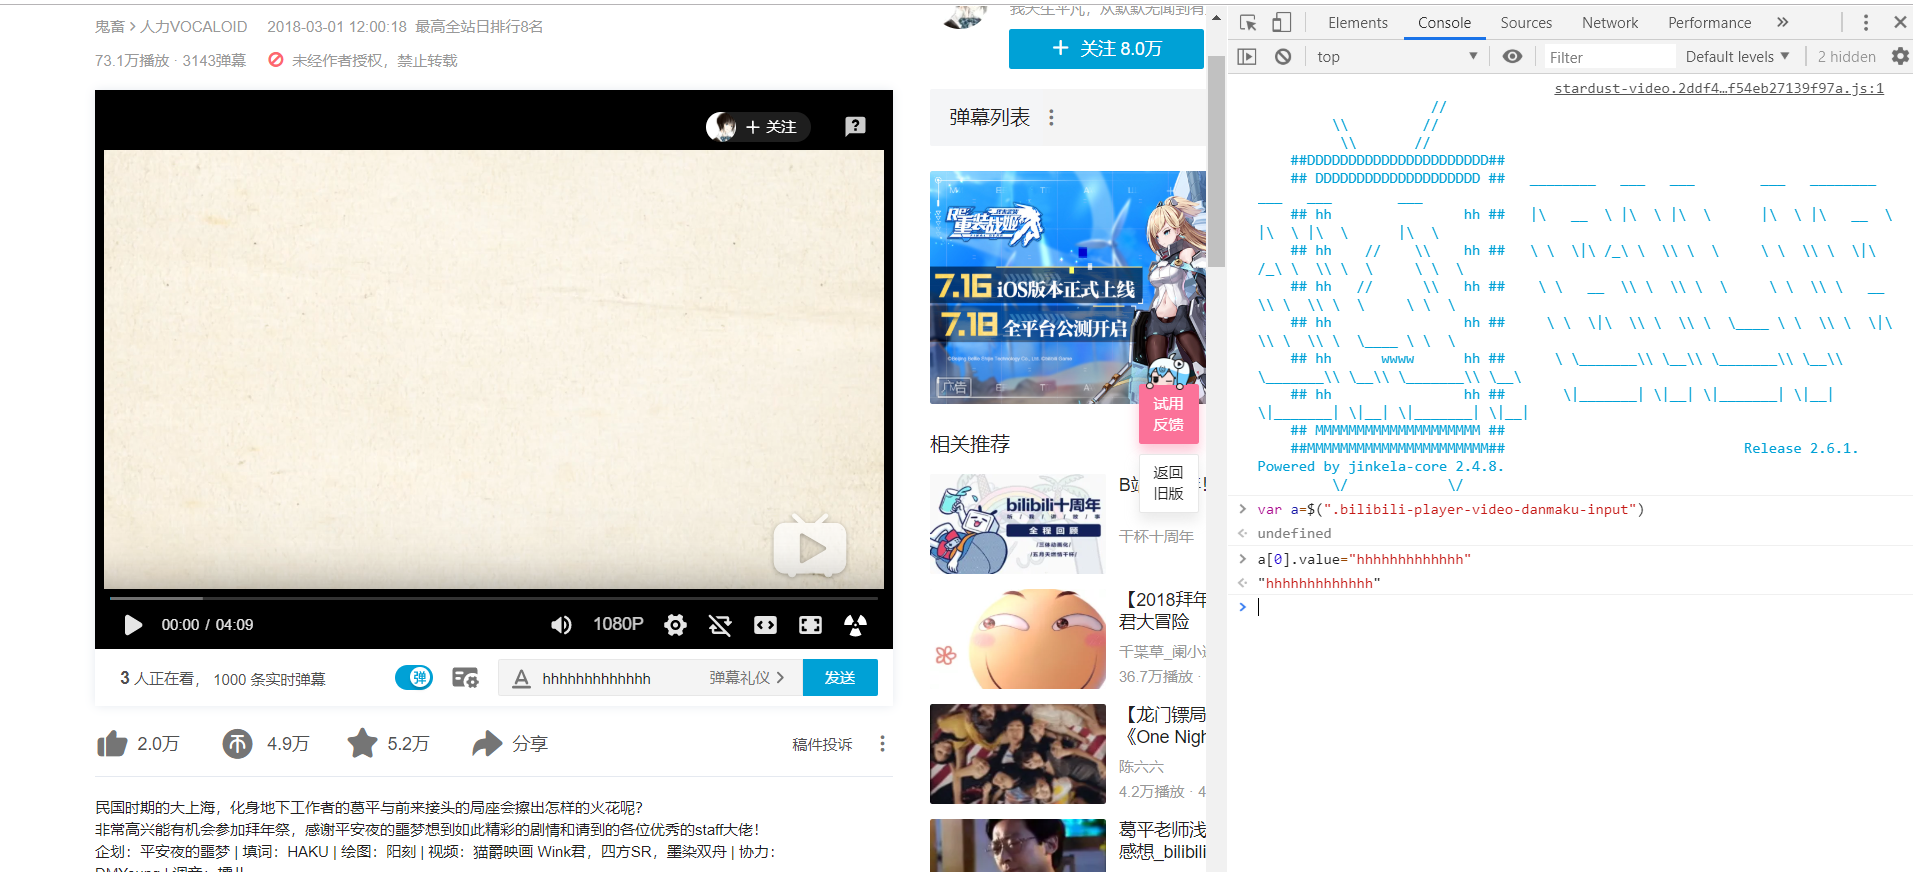
\includegraphics[scale=0.3]{06-27_4.png}
            \item[2.2] 
            之后利用类选择器找到提交按钮并触发它的点击事件\\
            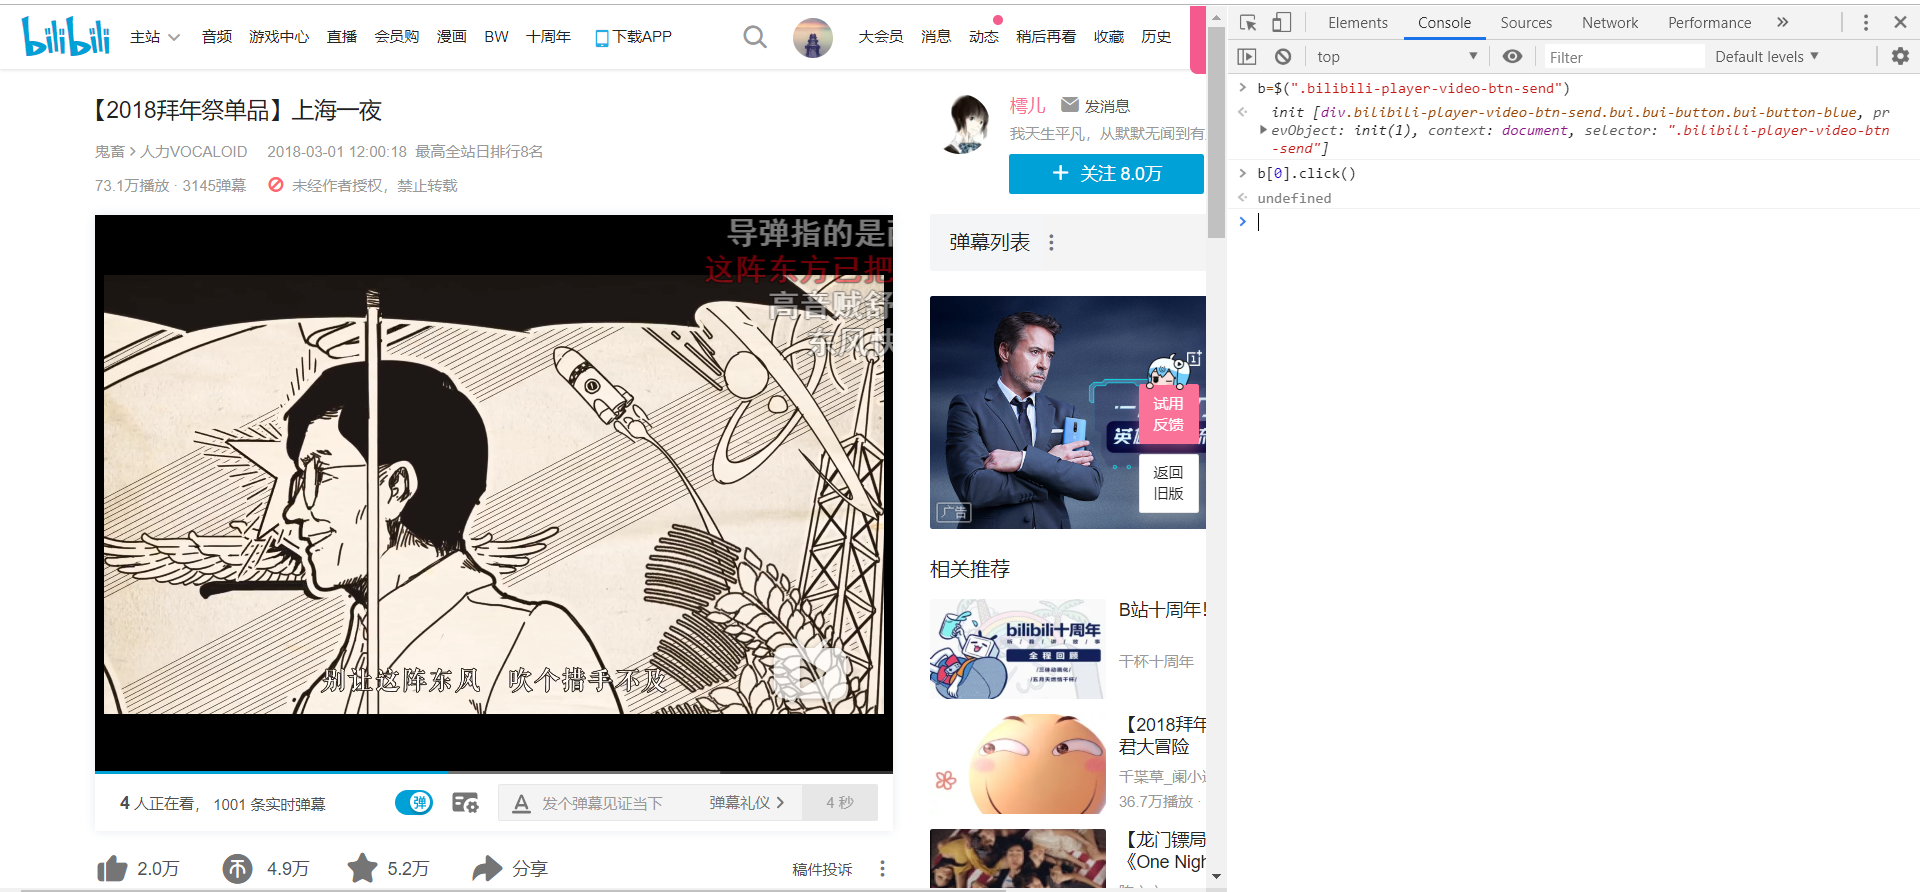
\includegraphics[scale=0.3]{06-27_5.png}
            \item[2.3] 
            我们再尝试通过控制台播放视频\\
            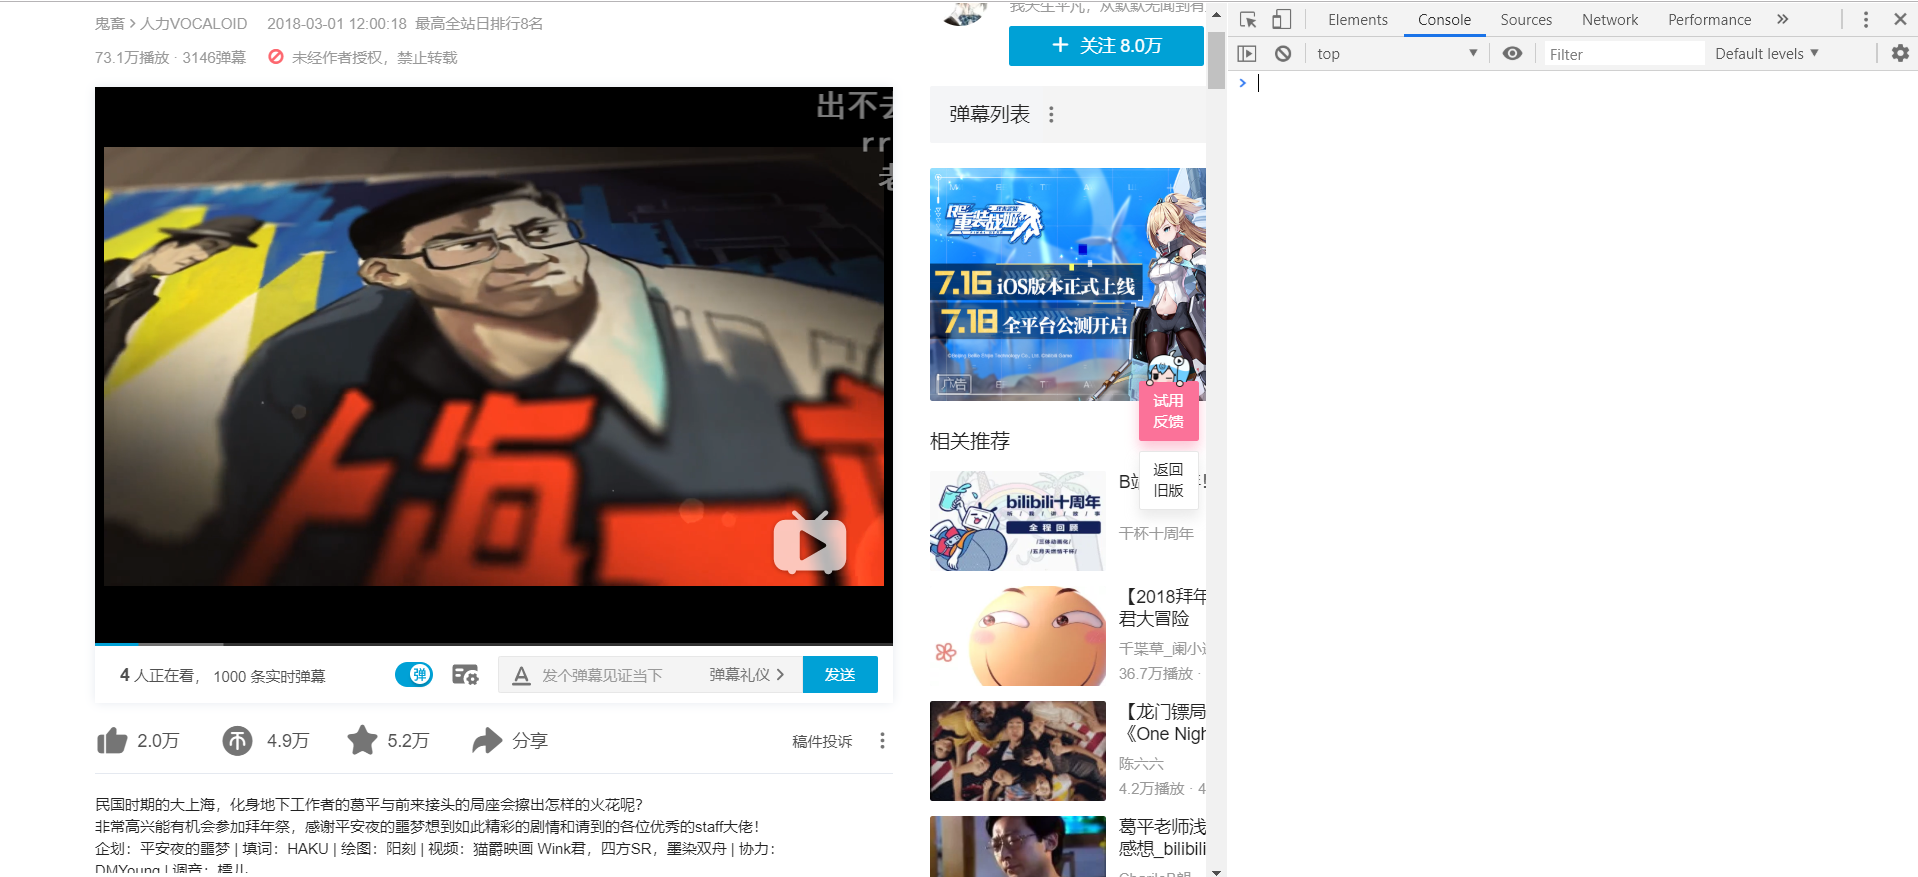
\includegraphics[scale=0.3]{06-27_6.png}
            由于网页中的video标签没有类和id不好确定我们为其手动添加id为``player-video'',
            然后利用id选择器找到id并播放视频,效果如下\\
            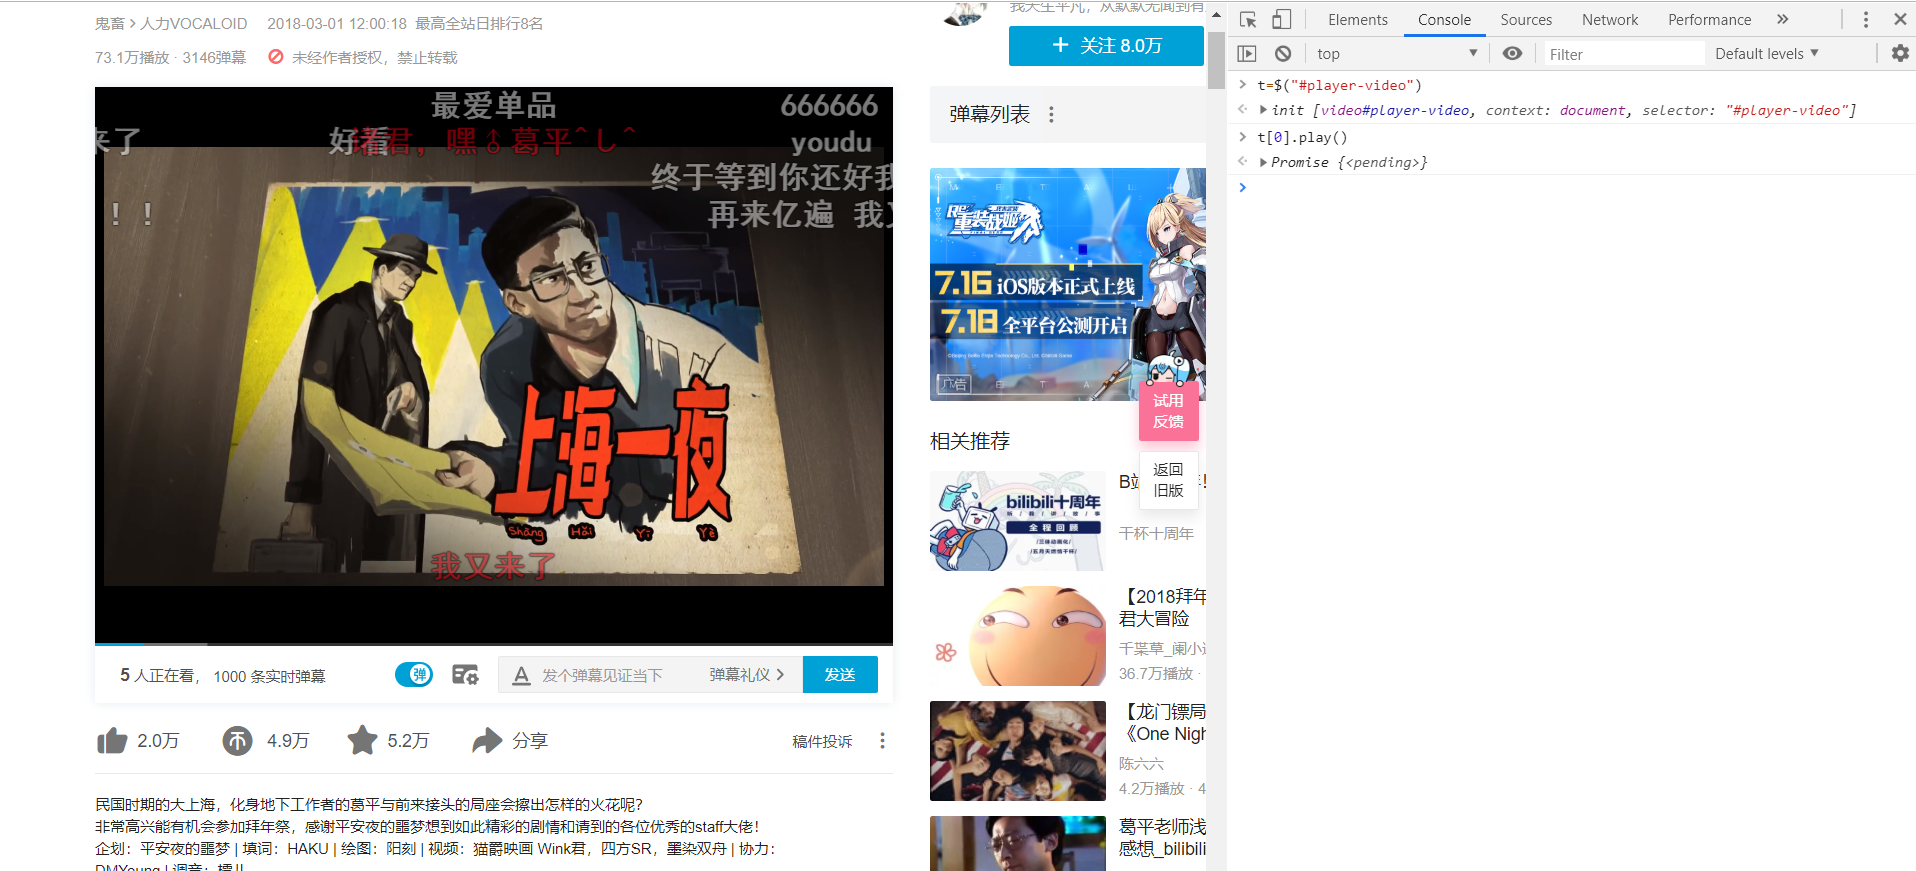
\includegraphics[scale=0.3]{06-27_7.png}  
        \end{enumerate} 
    \end{enumerate}
\end{document}